\section{Related Work}

\subsection{Music Theory Applications}
A search online and of the Apple ``App Store'' revealed several examples of applications which teach music theory, however none of these focus on writing music and are more based around ideas like flashcards and memorisation.

\begin{figure}[h!]
  \centering
  \frame{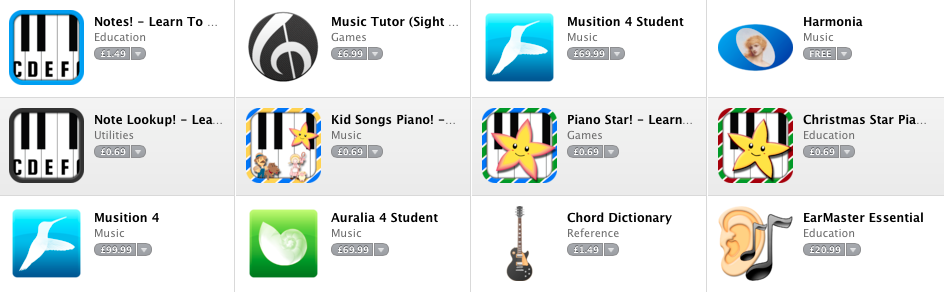
\includegraphics[width=\linewidth]{gfx/music-theory-apps.png}}
  \caption{Music Theory Applications after searching ``Music Theory'' on the Apple App Store}
\end{figure}

Most of these apps however, are aimed at more advanced students and miss out a huge part of theory exams which is the written notation section.

\subsection{Music Theory Workbooks}

\subsection{OMR Applications}
\subsubsection{Audiveris}
From the Audiveris site\footnote{https://audiveris.kenai.com/}:
\begin{quotation}
Audiveris is an open-source Optical Music Recognition software which processes the image of a music sheet to automatically provide symbolic music information in MusicXML standard.
\end{quotation}

At present it only supports high quality printed scores and operates by utilising a neural network which must be trained on samples by the end user.

\todo[inline]{Reference more commercial OMR applications}

